\title{Lausnir á völdum dæmum úr viku tvö}
\author{Bergur Snorrason}
\date{\today}

\begin{document}

\frame{\titlepage}

\env{frame}
{
	\env{itemize}
	{
		\item<1-> Ég mun leysa eftirfarandi dæmi:
		\env{itemize}
		{
			\item<2-> \emph{Reiknirit},
			\item<3-> \emph{Pipe Rotation},
			\item<4-> \emph{Language Survey}.
		}
	}
}

\env{frame}
{
	\frametitle{Reiknirit}
	\env{itemize}
	{
		\item<1-> Skoðum aftur skiladæmið \emph{Reiknirit}.
		\item<2-> Fyrsta lína inntaksins inniheldur heiltölu $n$.
		\item<3-> Síðan koma $n$ heiltölur $a_1, a_2, \dots, a_n$.
		\item<4-> Gerum ráð fyrir að við séum með forrit sem gerir eftirfarandi:
		\env{itemize}
		{
			\item<5-> Prentar tölurnar.
			\item<6-> Fjarlægir öll eintök af algengustu tölunni í listan.
			\item<7-> Endurtekur skrefin að ofan þar til listinn er tómur.
		}
		\item<8-> Dæmið snýst um að finna hversu margar tölur eru prentaðar í heildina.
	}
}

\env{frame}
{
	\frametitle{Reiknirit}
	\env{itemize}
	{
		\item<1-> Síðast leystum við þetta dæmi með því að útfæra forritið sem er lýst í dæminu.
		\item<2-> Við komumst þó að því að sú lausn var $\mathcal{O}(n^2)$ sem reyndist of hæg.
		\item<3-> Tökum eftir að við getum notað svipaða hugmynd og í hægu útfærslunni til að telja hversu oft hver tala kemur fyrir.
		\item<4-> Tökum einnig eftir að hvert eintak af algengustu tölunni er prentað einu sinni,
					hvert eintak af næst algengustu tölunni er prentað tvisvar
					og svo framvegis.
		\item<5-> Einnig skiptir talan sjálf ekki máli, heldur eingöngu hversu oft hún kemur fyrir.
	}
}

\env{frame}
{
	\frametitle{Reiknirit}
	\env{itemize}
	{
		\item<1-> Látum því $h_1 \geq h_2 \geq \dots \geq h_k$ þannig að algengast talan kemur $h_1$ sinni fyrir,
					næst algengasta talan kemur $h_2$ sinnum fyrir
					og svo framvegis.
		\item<2-> Svarið er því
		\[
			\sum_{i = 1}^k i \cdot h_i.
		\]
		\item<3-> Við þurfum þó að passa okkur aðeins.
		\item<4-> Ef $h_1 = h_2 = \dots h_k = 1$ (þá er einnig $k = n$) fæst að svarið er
		\[
			\sum_{i = 1}^k i \cdot h_i
			=
			\sum_{i = 1}^k i
			=
			\frac{n \cdot (n + 1)}{2}.
		\]
		\item<5-> Svo, þar sem $n$ getur verið allt að $10^6$, getur svarið okkar orðið of stórt fyrir \texttt{int}.
		\item<6-> Við þurfum því að nota \texttt{long long}.
	}
}

\env{frame}
{
	\frametitle{Reiknirit}
	\code{code/reiknirit.c}
}

\env{frame}
{
	\frametitle{Reiknirit}
	\env{itemize}
	{
		\item<1-> Sjáum við byrjum á að raða, sem er $\mathcal{O}($\onslide<2->{$n \log n$}$)$.
		\item<3-> Við teljum síðan hvað hver tala kemur oft fyrir, sem er $\mathcal{O}($\onslide<4->{$\ n\ $}$)$.
		\item<5-> Síðan röðum við aftur.
		\item<6-> Að lokum reiknum við summuna í $\mathcal{O}($\onslide<7->{$\ n\ $}$)$.
		\item<8-> Tímaflækjan er því í heildina $\mathcal{O}($\onslide<9->{$n \log n$}$)$.
		\item<10-> Nú er $10^{-8} \cdot 10^6 \cdot \log 10^6 \sim 0,2$, svo þessi lausn er nógu hröð.
	}
}

\env{frame}
{
	\frametitle{Pipe Rotation}
	\env{itemize}
	{
		\item<1-> Okkur er gefið $n \times m$ ($1 \leq n, m \leq 100$) borð af spilum af eftirfarandi gerðum:
		\item<2->[] 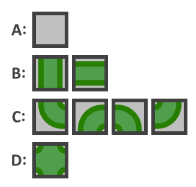
\includegraphics[scale = 0.25]{fig/pr1}
		\item<3-> Við eigum að ákvarða hvort hægt sé að snúa spilunum þannig að allar hliðar sem eru grænar eru gagnstæðar hliðum sem eru einnig grænar.
		\item<4-> Takið eftir að við megum ekki endurraða spilunum og að hliðar sem snúa út mega ekki vera grænar.
	}
}

\env{frame}
{
	\frametitle{Pipe Rotation}
	\env{itemize}
	{
		\item<1-> Sjáum dæmi.
		\item<2->[] 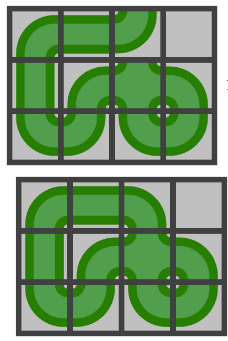
\includegraphics[scale = 0.25]{fig/pr2}
		\item<3-> Efra dæmið er ekki löglegt en neðra er löglegt.
	}
}

\env{frame}
{
	\frametitle{Pipe Rotation}
	\env{columns}
	{
		\env{column}
		{
			{0.8\textwidth}
			\env{itemize}
			{
				\item<1-> Sjáum fyrst að ef við vitum hvað er vinstra megin og fyrir ofan spil þá vitum við hvernig það þarf að snúa.
				\item<2-> Ef hliðin fyrir ofan er auð og hliðin til vinstri er auð þá þarf spilið að vera af gerð \texttt{A}
							eða af gerð \texttt{C} í öðrum snúning.
				\item<3-> Ef hliðin fyrir ofan er auð og hliðin til vinstri er græn þá þarf spilið að vera af gerð \texttt{B} í seinni snúning
							eða af gerð \texttt{C} í þriðja snúning.
				\item<4-> Ef hliðin fyrir ofan er græn og hliðin til vinstri er auð þá þarf spilið að vera af gerð \texttt{B} í fyrri snúning
							eða af gerð \texttt{C} í fyrsta snúning.
				\item<5-> Ef hliðin fyrir ofan er græn og hliðin til vinstri er græn þá þarf spilið að vera af gerð \texttt{C} í fjórða snúning
							eða af gerð \texttt{D}.
			}
		}
		\env{column}
		{
			{0.2\textwidth}
			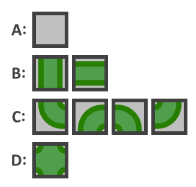
\includegraphics[scale = 0.3]{fig/pr1}
		}
	}
}

\env{frame}
{
	\frametitle{Pipe Rotation}
	\env{itemize}
	{
		\item<1-> Nú getum við labbað í gegnum öll spilin og ákvarðað hvernig hvert spil snýr ef við byrjum á efstu línunni og vinnum okkur niður,
					og skoðum hverja línu frá vinstri til hægri.
		\item<2-> Það er pínu vinna að útfæra þetta útaf öllum tilfellunum sem þarf að hafa í huga.
	}
}

\env{frame}
{
	\selectcode{code/piperotation.c}{4}{8}
}

\env{frame}
{
	\selectcode{code/piperotation.c}{10}{47}
}

\env{frame}
{
	\frametitle{Pipe Rotation}
	\env{itemize}
	{
		\item<1-> Þessi lausn er lítið annað en tvöföld \texttt{for}-lykkja sú ytri af lengd $n$ og sú innri af lengd $m$.
		\item<2-> Svo tímaflækjan er $\mathcal{O}($\onslide<3->{$n \cdot m$}$)$.
	}
}

\env{frame}
{
	\frametitle{Language Survey}
	\env{itemize}
	{
		\item<1-> Þér er gefið land sem er skipt í grind eftir hvaða tungumál eru töluð hvar.
		\item<2-> Þú veist að í heildina eru þrjú tungumál töluð.
		\item<3-> Þér er einnig sagt, fyrir sérhvern reit, hvort eitt tungumál er talað þar eða fleiri.
		\item<4-> Einnig er gefið að hvert tungumál er talað á samanhangandi svæði reita.
		\item<5-> Með öðrum orðum getur þú labbað milli allra reita sem tala sama tungumál án þess að þurfa að heimsækja reit sem talar ekki tungumálið.
	}
}

\env{frame}
{
	\frametitle{Language Survey}
	\env{itemize}
	{
		\item<1-> Fyrra sýniinntakið er
		\item<2->[] \code{code/languagesurvey.01.in}
		\item<3-> og samsvarandi úttak er
		\item<4->[]\code{code/languagesurvey.01.ans}
	}
}

\env{frame}
{
	\frametitle{Language Survey}
	\env{itemize}
	{
		\item<1-> Gerum ráð fyrir að við getum raðað tungumálunum þannig að eitt tungumál er talað í hverjum reit,
					en fyrir hvern reit er líka, að minnsta kosti, einn nágranni sem talar annað tungumál.
		\item<2-> Ef slík skipun er til þá er eftirleikurinn auðveldur.
		\item<3-> Fyrir hvern reit þar sem fleiri en eitt tungumál er talað veljum við tungumálið sem er talað hjá nágrannanum sem talar annað tungumál
					og látum það tungumál líka talað í þeim reit.
		\item<4-> En er slík skipun til?
	}
}

\env{frame}
{
	\frametitle{Language Survey}
	\env{itemize}
	{
		\item<1-> Byrjum á að láta dálkinn lengst til vinstri fá tungumál \texttt{A}.
		\item<2-> Við látum svo \texttt{p} tákna reitinn efst til hægri og \texttt{q} tákna reitinn neðst til hægri og:
		\env{itemize}
		{
			\item<3-> Færum \texttt{p} til vintri þangað til hann kemst ekki lengra og látum alla reiti sem hann lendir á fá tungumál \texttt{B}.
			\item<4-> Færum \texttt{p} niður þangað til hann kemst ekki lengra og látum alla reiti sem hann lendir á fá tungumál \texttt{B}.
			\item<5-> Færum \texttt{q} upp þangað til hann kemst ekki lengra og látum alla reiti sem hann lendir á fá tungumál \texttt{C}.
			\item<6-> Færum \texttt{q} til vinstri þangað til hann kemst ekki lengra og látum alla reiti sem hann lendir á fá tungumál \texttt{C}.
			\item<7-> Færum \texttt{p} til hægri þangað til hann kemst ekki lengra og látum alla reiti sem hann lendir á fá tungumál \texttt{B}.
			\item<8-> Færum \texttt{p} upp þangað til hann kemst ekki lengra og látum alla reiti sem hann lendir á fá tungumál \texttt{B}.
			\item<9-> Færum \texttt{q} niður þangað til hann kemst ekki lengra og látum alla reiti sem hann lendir á fá tungumál \texttt{C}.
			\item<10-> Færum \texttt{q} til hægri þangað til hann kemst ekki lengra og látum alla reiti sem hann lendir á fá tungumál \texttt{C}.
			\item<11-> Endurtökum þar til allir reitir hafa tungumál.
		}
	}
}

\defverbatim{\langAA}
{ \begin{verbatim}
         x x x x x x x x x
         x x x x x x x x x
         x x x x x x x x x
         x x x x x x x x x
         x x x x x x x x x
         x x x x x x x x x
         x x x x x x x x x
         x x x x x x x x x
         x x x x x x x x x
\end{verbatim} }

\defverbatim{\langAB}
{ \begin{verbatim}
         A x x x x x x x x
         A x x x x x x x x
         A x x x x x x x x
         A x x x x x x x x
         A x x x x x x x x
         A x x x x x x x x
         A x x x x x x x x
         A x x x x x x x x
         A x x x x x x x x
\end{verbatim} }

\defverbatim{\langAC}
{ \begin{verbatim}
         A x x x x x x x B
         A x x x x x x x x
         A x x x x x x x x
         A x x x x x x x x
         A x x x x x x x x
         A x x x x x x x x
         A x x x x x x x x
         A x x x x x x x x
         A x x x x x x x x
\end{verbatim} }

\defverbatim{\langAD}
{ \begin{verbatim}
         A x x x x x x B B
         A x x x x x x x x
         A x x x x x x x x
         A x x x x x x x x
         A x x x x x x x x
         A x x x x x x x x
         A x x x x x x x x
         A x x x x x x x x
         A x x x x x x x x
\end{verbatim} }

\defverbatim{\langAE}
{ \begin{verbatim}
         A x x x x x B B B
         A x x x x x x x x
         A x x x x x x x x
         A x x x x x x x x
         A x x x x x x x x
         A x x x x x x x x
         A x x x x x x x x
         A x x x x x x x x
         A x x x x x x x x
\end{verbatim} }

\defverbatim{\langAF}
{ \begin{verbatim}
         A x x x x B B B B
         A x x x x x x x x
         A x x x x x x x x
         A x x x x x x x x
         A x x x x x x x x
         A x x x x x x x x
         A x x x x x x x x
         A x x x x x x x x
         A x x x x x x x x
\end{verbatim} }

\defverbatim{\langAG}
{ \begin{verbatim}
         A x x x B B B B B
         A x x x x x x x x
         A x x x x x x x x
         A x x x x x x x x
         A x x x x x x x x
         A x x x x x x x x
         A x x x x x x x x
         A x x x x x x x x
         A x x x x x x x x
\end{verbatim} }

\defverbatim{\langAH}
{ \begin{verbatim}
         A x x B B B B B B
         A x x x x x x x x
         A x x x x x x x x
         A x x x x x x x x
         A x x x x x x x x
         A x x x x x x x x
         A x x x x x x x x
         A x x x x x x x x
         A x x x x x x x x
\end{verbatim} }

\defverbatim{\langAI}
{ \begin{verbatim}
         A x B B B B B B B
         A x x x x x x x x
         A x x x x x x x x
         A x x x x x x x x
         A x x x x x x x x
         A x x x x x x x x
         A x x x x x x x x
         A x x x x x x x x
         A x x x x x x x x
\end{verbatim} }

\defverbatim{\langAJ}
{ \begin{verbatim}
         A B B B B B B B B
         A x x x x x x x x
         A x x x x x x x x
         A x x x x x x x x
         A x x x x x x x x
         A x x x x x x x x
         A x x x x x x x x
         A x x x x x x x x
         A x x x x x x x x
\end{verbatim} }

\defverbatim{\langAK}
{ \begin{verbatim}
         A B B B B B B B B
         A B x x x x x x x
         A x x x x x x x x
         A x x x x x x x x
         A x x x x x x x x
         A x x x x x x x x
         A x x x x x x x x
         A x x x x x x x x
         A x x x x x x x x
\end{verbatim} }

\defverbatim{\langAL}
{ \begin{verbatim}
         A B B B B B B B B
         A B x x x x x x x
         A B x x x x x x x
         A x x x x x x x x
         A x x x x x x x x
         A x x x x x x x x
         A x x x x x x x x
         A x x x x x x x x
         A x x x x x x x x
\end{verbatim} }

\defverbatim{\langAM}
{ \begin{verbatim}
         A B B B B B B B B
         A B x x x x x x x
         A B x x x x x x x
         A B x x x x x x x
         A x x x x x x x x
         A x x x x x x x x
         A x x x x x x x x
         A x x x x x x x x
         A x x x x x x x x
\end{verbatim} }

\defverbatim{\langAN}
{ \begin{verbatim}
         A B B B B B B B B
         A B x x x x x x x
         A B x x x x x x x
         A B x x x x x x x
         A B x x x x x x x
         A x x x x x x x x
         A x x x x x x x x
         A x x x x x x x x
         A x x x x x x x x
\end{verbatim} }

\defverbatim{\langAO}
{ \begin{verbatim}
         A B B B B B B B B
         A B x x x x x x x
         A B x x x x x x x
         A B x x x x x x x
         A B x x x x x x x
         A B x x x x x x x
         A x x x x x x x x
         A x x x x x x x x
         A x x x x x x x x
\end{verbatim} }

\defverbatim{\langAP}
{ \begin{verbatim}
         A B B B B B B B B
         A B x x x x x x x
         A B x x x x x x x
         A B x x x x x x x
         A B x x x x x x x
         A B x x x x x x x
         A B x x x x x x x
         A x x x x x x x x
         A x x x x x x x x
\end{verbatim} }

\defverbatim{\langAQ}
{ \begin{verbatim}
         A B B B B B B B B
         A B x x x x x x x
         A B x x x x x x x
         A B x x x x x x x
         A B x x x x x x x
         A B x x x x x x x
         A B x x x x x x x
         A B x x x x x x x
         A x x x x x x x x
\end{verbatim} }

\defverbatim{\langAR}
{ \begin{verbatim}
         A B B B B B B B B
         A B x x x x x x x
         A B x x x x x x x
         A B x x x x x x x
         A B x x x x x x x
         A B x x x x x x x
         A B x x x x x x x
         A B x x x x x x x
         A B x x x x x x x
\end{verbatim} }

\defverbatim{\langARR}
{ \begin{verbatim}
         A B B B B B B B B
         A B x x x x x x x
         A B x x x x x x x
         A B x x x x x x x
         A B x x x x x x x
         A B x x x x x x x
         A B x x x x x x x
         A B x x x x x x x
         A B x x x x x x C
\end{verbatim} }

\defverbatim{\langAS}
{ \begin{verbatim}
         A B B B B B B B B
         A B x x x x x x x
         A B x x x x x x x
         A B x x x x x x x
         A B x x x x x x x
         A B x x x x x x x
         A B x x x x x x x
         A B x x x x x x C
         A B x x x x x x C
\end{verbatim} }

\defverbatim{\langAT}
{ \begin{verbatim}
         A B B B B B B B B
         A B x x x x x x x
         A B x x x x x x x
         A B x x x x x x x
         A B x x x x x x x
         A B x x x x x x x
         A B x x x x x x C
         A B x x x x x x C
         A B x x x x x x C
\end{verbatim} }

\defverbatim{\langAU}
{ \begin{verbatim}
         A B B B B B B B B
         A B x x x x x x x
         A B x x x x x x x
         A B x x x x x x x
         A B x x x x x x x
         A B x x x x x x C
         A B x x x x x x C
         A B x x x x x x C
         A B x x x x x x C
\end{verbatim} }

\defverbatim{\langAV}
{ \begin{verbatim}
         A B B B B B B B B
         A B x x x x x x x
         A B x x x x x x x
         A B x x x x x x x
         A B x x x x x x C
         A B x x x x x x C
         A B x x x x x x C
         A B x x x x x x C
         A B x x x x x x C
\end{verbatim} }

\defverbatim{\langAW}
{ \begin{verbatim}
         A B B B B B B B B
         A B x x x x x x x
         A B x x x x x x x
         A B x x x x x x C
         A B x x x x x x C
         A B x x x x x x C
         A B x x x x x x C
         A B x x x x x x C
         A B x x x x x x C
\end{verbatim} }

\defverbatim{\langAX}
{ \begin{verbatim}
         A B B B B B B B B
         A B x x x x x x x
         A B x x x x x x C
         A B x x x x x x C
         A B x x x x x x C
         A B x x x x x x C
         A B x x x x x x C
         A B x x x x x x C
         A B x x x x x x C
\end{verbatim} }

\defverbatim{\langAY}
{ \begin{verbatim}
         A B B B B B B B B
         A B x x x x x x C
         A B x x x x x x C
         A B x x x x x x C
         A B x x x x x x C
         A B x x x x x x C
         A B x x x x x x C
         A B x x x x x x C
         A B x x x x x x C
\end{verbatim} }

\defverbatim{\langAZ}
{ \begin{verbatim}
         A B B B B B B B B
         A B x x x x x C C
         A B x x x x x x C
         A B x x x x x x C
         A B x x x x x x C
         A B x x x x x x C
         A B x x x x x x C
         A B x x x x x x C
         A B x x x x x x C
\end{verbatim} }

\defverbatim{\langBA}
{ \begin{verbatim}
         A B B B B B B B B
         A B x x x x C C C
         A B x x x x x x C
         A B x x x x x x C
         A B x x x x x x C
         A B x x x x x x C
         A B x x x x x x C
         A B x x x x x x C
         A B x x x x x x C
\end{verbatim} }

\defverbatim{\langBB}
{ \begin{verbatim}
         A B B B B B B B B
         A B x x x C C C C
         A B x x x x x x C
         A B x x x x x x C
         A B x x x x x x C
         A B x x x x x x C
         A B x x x x x x C
         A B x x x x x x C
         A B x x x x x x C
\end{verbatim} }

\defverbatim{\langBC}
{ \begin{verbatim}
         A B B B B B B B B
         A B x x C C C C C
         A B x x x x x x C
         A B x x x x x x C
         A B x x x x x x C
         A B x x x x x x C
         A B x x x x x x C
         A B x x x x x x C
         A B x x x x x x C
\end{verbatim} }

\defverbatim{\langBD}
{ \begin{verbatim}
         A B B B B B B B B
         A B x C C C C C C
         A B x x x x x x C
         A B x x x x x x C
         A B x x x x x x C
         A B x x x x x x C
         A B x x x x x x C
         A B x x x x x x C
         A B x x x x x x C
\end{verbatim} }

\defverbatim{\langBE}
{ \begin{verbatim}
         A B B B B B B B B
         A B C C C C C C C
         A B x x x x x x C
         A B x x x x x x C
         A B x x x x x x C
         A B x x x x x x C
         A B x x x x x x C
         A B x x x x x x C
         A B x x x x x x C
\end{verbatim} }

\defverbatim{\langBF}
{ \begin{verbatim}
         A B B B B B B B B
         A B C C C C C C C
         A B x x x x x x C
         A B x x x x x x C
         A B x x x x x x C
         A B x x x x x x C
         A B x x x x x x C
         A B x x x x x x C
         A B B x x x x x C
\end{verbatim} }

\defverbatim{\langBG}
{ \begin{verbatim}
         A B B B B B B B B
         A B C C C C C C C
         A B x x x x x x C
         A B x x x x x x C
         A B x x x x x x C
         A B x x x x x x C
         A B x x x x x x C
         A B x x x x x x C
         A B B B x x x x C
\end{verbatim} }

\defverbatim{\langBH}
{ \begin{verbatim}
         A B B B B B B B B
         A B C C C C C C C
         A B x x x x x x C
         A B x x x x x x C
         A B x x x x x x C
         A B x x x x x x C
         A B x x x x x x C
         A B x x x x x x C
         A B B B B x x x C
\end{verbatim} }

\defverbatim{\langBI}
{ \begin{verbatim}
         A B B B B B B B B
         A B C C C C C C C
         A B x x x x x x C
         A B x x x x x x C
         A B x x x x x x C
         A B x x x x x x C
         A B x x x x x x C
         A B x x x x x x C
         A B B B B B x x C
\end{verbatim} }

\defverbatim{\langBJ}
{ \begin{verbatim}
         A B B B B B B B B
         A B C C C C C C C
         A B x x x x x x C
         A B x x x x x x C
         A B x x x x x x C
         A B x x x x x x C
         A B x x x x x x C
         A B x x x x x x C
         A B B B B B B x C
\end{verbatim} }

\defverbatim{\langBK}
{ \begin{verbatim}
         A B B B B B B B B
         A B C C C C C C C
         A B x x x x x x C
         A B x x x x x x C
         A B x x x x x x C
         A B x x x x x x C
         A B x x x x x x C
         A B x x x x x x C
         A B B B B B B B C
\end{verbatim} }

\defverbatim{\langBL}
{ \begin{verbatim}
         A B B B B B B B B
         A B C C C C C C C
         A B x x x x x x C
         A B x x x x x x C
         A B x x x x x x C
         A B x x x x x x C
         A B x x x x x x C
         A B x x x x x B C
         A B B B B B B B C
\end{verbatim} }

\defverbatim{\langBM}
{ \begin{verbatim}
         A B B B B B B B B
         A B C C C C C C C
         A B x x x x x x C
         A B x x x x x x C
         A B x x x x x x C
         A B x x x x x x C
         A B x x x x x B C
         A B x x x x x B C
         A B B B B B B B C
\end{verbatim} }

\defverbatim{\langBN}
{ \begin{verbatim}
         A B B B B B B B B
         A B C C C C C C C
         A B x x x x x x C
         A B x x x x x x C
         A B x x x x x x C
         A B x x x x x B C
         A B x x x x x B C
         A B x x x x x B C
         A B B B B B B B C
\end{verbatim} }

\defverbatim{\langBO}
{ \begin{verbatim}
         A B B B B B B B B
         A B C C C C C C C
         A B x x x x x x C
         A B x x x x x x C
         A B x x x x x B C
         A B x x x x x B C
         A B x x x x x B C
         A B x x x x x B C
         A B B B B B B B C
\end{verbatim} }

\defverbatim{\langBP}
{ \begin{verbatim}
         A B B B B B B B B
         A B C C C C C C C
         A B x x x x x x C
         A B x x x x x B C
         A B x x x x x B C
         A B x x x x x B C
         A B x x x x x B C
         A B x x x x x B C
         A B B B B B B B C
\end{verbatim} }

\defverbatim{\langBQ}
{ \begin{verbatim}
         A B B B B B B B B
         A B C C C C C C C
         A B x x x x x B C
         A B x x x x x B C
         A B x x x x x B C
         A B x x x x x B C
         A B x x x x x B C
         A B x x x x x B C
         A B B B B B B B C
\end{verbatim} }

\defverbatim{\langBR}
{ \begin{verbatim}
         A B B B B B B B B
         A B C C C C C C C
         A B C x x x x B C
         A B x x x x x B C
         A B x x x x x B C
         A B x x x x x B C
         A B x x x x x B C
         A B x x x x x B C
         A B B B B B B B C
\end{verbatim} }

\defverbatim{\langBS}
{ \begin{verbatim}
         A B B B B B B B B
         A B C C C C C C C
         A B C x x x x B C
         A B C x x x x B C
         A B x x x x x B C
         A B x x x x x B C
         A B x x x x x B C
         A B x x x x x B C
         A B B B B B B B C
\end{verbatim} }

\defverbatim{\langBT}
{ \begin{verbatim}
         A B B B B B B B B
         A B C C C C C C C
         A B C x x x x B C
         A B C x x x x B C
         A B C x x x x B C
         A B x x x x x B C
         A B x x x x x B C
         A B x x x x x B C
         A B B B B B B B C
\end{verbatim} }

\defverbatim{\langBU}
{ \begin{verbatim}
         A B B B B B B B B
         A B C C C C C C C
         A B C x x x x B C
         A B C x x x x B C
         A B C x x x x B C
         A B C x x x x B C
         A B x x x x x B C
         A B x x x x x B C
         A B B B B B B B C
\end{verbatim} }

\defverbatim{\langBV}
{ \begin{verbatim}
         A B B B B B B B B
         A B C C C C C C C
         A B C x x x x B C
         A B C x x x x B C
         A B C x x x x B C
         A B C x x x x B C
         A B C x x x x B C
         A B x x x x x B C
         A B B B B B B B C
\end{verbatim} }

\defverbatim{\langBW}
{ \begin{verbatim}
         A B B B B B B B B
         A B C C C C C C C
         A B C x x x x B C
         A B C x x x x B C
         A B C x x x x B C
         A B C x x x x B C
         A B C x x x x B C
         A B C x x x x B C
         A B B B B B B B C
\end{verbatim} }

\defverbatim{\langBX}
{ \begin{verbatim}
         A B B B B B B B B
         A B C C C C C C C
         A B C x x x x B C
         A B C x x x x B C
         A B C x x x x B C
         A B C x x x x B C
         A B C x x x x B C
         A B C C x x x B C
         A B B B B B B B C
\end{verbatim} }

\defverbatim{\langBY}
{ \begin{verbatim}
         A B B B B B B B B
         A B C C C C C C C
         A B C x x x x B C
         A B C x x x x B C
         A B C x x x x B C
         A B C x x x x B C
         A B C x x x x B C
         A B C C C x x B C
         A B B B B B B B C
\end{verbatim} }

\defverbatim{\langBYY}
{ \begin{verbatim}
         A B B B B B B B B
         A B C C C C C C C
         A B C x x x x B C
         A B C x x x x B C
         A B C x x x x B C
         A B C x x x x B C
         A B C x x x x B C
         A B C C C C x B C
         A B B B B B B B C
\end{verbatim} }

\defverbatim{\langBZ}
{ \begin{verbatim}
         A B B B B B B B B
         A B C C C C C C C
         A B C x x x x B C
         A B C x x x x B C
         A B C x x x x B C
         A B C x x x x B C
         A B C x x x x B C
         A B C C C C C B C
         A B B B B B B B C
\end{verbatim} }

\defverbatim{\langCA}
{ \begin{verbatim}
         A B B B B B B B B
         A B C C C C C C C
         A B C x x x B B C
         A B C x x x x B C
         A B C x x x x B C
         A B C x x x x B C
         A B C x x x x B C
         A B C C C C C B C
         A B B B B B B B C
\end{verbatim} }

\defverbatim{\langCB}
{ \begin{verbatim}
         A B B B B B B B B
         A B C C C C C C C
         A B C x x B B B C
         A B C x x x x B C
         A B C x x x x B C
         A B C x x x x B C
         A B C x x x x B C
         A B C C C C C B C
         A B B B B B B B C
\end{verbatim} }

\defverbatim{\langCC}
{ \begin{verbatim}
         A B B B B B B B B
         A B C C C C C C C
         A B C x B B B B C
         A B C x x x x B C
         A B C x x x x B C
         A B C x x x x B C
         A B C x x x x B C
         A B C C C C C B C
         A B B B B B B B C
\end{verbatim} }

\defverbatim{\langCD}
{ \begin{verbatim}
         A B B B B B B B B
         A B C C C C C C C
         A B C B B B B B C
         A B C x x x x B C
         A B C x x x x B C
         A B C x x x x B C
         A B C x x x x B C
         A B C C C C C B C
         A B B B B B B B C
\end{verbatim} }

\defverbatim{\langCE}
{ \begin{verbatim}
         A B B B B B B B B
         A B C C C C C C C
         A B C B B B B B C
         A B C B x x x B C
         A B C x x x x B C
         A B C x x x x B C
         A B C x x x x B C
         A B C C C C C B C
         A B B B B B B B C
\end{verbatim} }

\defverbatim{\langCF}
{ \begin{verbatim}
         A B B B B B B B B
         A B C C C C C C C
         A B C B B B B B C
         A B C B x x x B C
         A B C B x x x B C
         A B C x x x x B C
         A B C x x x x B C
         A B C C C C C B C
         A B B B B B B B C
\end{verbatim} }

\defverbatim{\langCG}
{ \begin{verbatim}
         A B B B B B B B B
         A B C C C C C C C
         A B C B B B B B C
         A B C B x x x B C
         A B C B x x x B C
         A B C B x x x B C
         A B C x x x x B C
         A B C C C C C B C
         A B B B B B B B C
\end{verbatim} }

\defverbatim{\langCH}
{ \begin{verbatim}
         A B B B B B B B B
         A B C C C C C C C
         A B C B B B B B C
         A B C B x x x B C
         A B C B x x x B C
         A B C B x x x B C
         A B C B x x x B C
         A B C C C C C B C
         A B B B B B B B C
\end{verbatim} }

\defverbatim{\langCI}
{ \begin{verbatim}
         A B B B B B B B B
         A B C C C C C C C
         A B C B B B B B C
         A B C B x x x B C
         A B C B x x x B C
         A B C B x x x B C
         A B C B x x C B C
         A B C C C C C B C
         A B B B B B B B C
\end{verbatim} }

\defverbatim{\langCJ}
{ \begin{verbatim}
         A B B B B B B B B
         A B C C C C C C C
         A B C B B B B B C
         A B C B x x x B C
         A B C B x x x B C
         A B C B x x C B C
         A B C B x x C B C
         A B C C C C C B C
         A B B B B B B B C
\end{verbatim} }

\defverbatim{\langCK}
{ \begin{verbatim}
         A B B B B B B B B
         A B C C C C C C C
         A B C B B B B B C
         A B C B x x x B C
         A B C B x x C B C
         A B C B x x C B C
         A B C B x x C B C
         A B C C C C C B C
         A B B B B B B B C
\end{verbatim} }

\defverbatim{\langCL}
{ \begin{verbatim}
         A B B B B B B B B
         A B C C C C C C C
         A B C B B B B B C
         A B C B x x C B C
         A B C B x x C B C
         A B C B x x C B C
         A B C B x x C B C
         A B C C C C C B C
         A B B B B B B B C
\end{verbatim} }

\defverbatim{\langCM}
{ \begin{verbatim}
         A B B B B B B B B
         A B C C C C C C C
         A B C B B B B B C
         A B C B x C C B C
         A B C B x x C B C
         A B C B x x C B C
         A B C B x x C B C
         A B C C C C C B C
         A B B B B B B B C
\end{verbatim} }

\defverbatim{\langCN}
{ \begin{verbatim}
         A B B B B B B B B
         A B C C C C C C C
         A B C B B B B B C
         A B C B C C C B C
         A B C B x x C B C
         A B C B x x C B C
         A B C B x x C B C
         A B C C C C C B C
         A B B B B B B B C
\end{verbatim} }

\defverbatim{\langCO}
{ \begin{verbatim}
         A B B B B B B B B
         A B C C C C C C C
         A B C B B B B B C
         A B C B C C C B C
         A B C B x x C B C
         A B C B x x C B C
         A B C B B x C B C
         A B C C C C C B C
         A B B B B B B B C
\end{verbatim} }

\defverbatim{\langCP}
{ \begin{verbatim}
         A B B B B B B B B
         A B C C C C C C C
         A B C B B B B B C
         A B C B C C C B C
         A B C B x x C B C
         A B C B x x C B C
         A B C B B B C B C
         A B C C C C C B C
         A B B B B B B B C
\end{verbatim} }

\defverbatim{\langCQ}
{ \begin{verbatim}
         A B B B B B B B B
         A B C C C C C C C
         A B C B B B B B C
         A B C B C C C B C
         A B C B x x C B C
         A B C B x B C B C
         A B C B B B C B C
         A B C C C C C B C
         A B B B B B B B C
\end{verbatim} }

\defverbatim{\langCR}
{ \begin{verbatim}
         A B B B B B B B B
         A B C C C C C C C
         A B C B B B B B C
         A B C B C C C B C
         A B C B x B C B C
         A B C B x B C B C
         A B C B B B C B C
         A B C C C C C B C
         A B B B B B B B C
\end{verbatim} }

\defverbatim{\langCS}
{ \begin{verbatim}
         A B B B B B B B B
         A B C C C C C C C
         A B C B B B B B C
         A B C B C C C B C
         A B C B C B C B C
         A B C B x B C B C
         A B C B B B C B C
         A B C C C C C B C
         A B B B B B B B C
\end{verbatim} }

\defverbatim{\langCT}
{ \begin{verbatim}
         A B B B B B B B B
         A B C C C C C C C
         A B C B B B B B C
         A B C B C C C B C
         A B C B C B C B C
         A B C B C B C B C
         A B C B B B C B C
         A B C C C C C B C
         A B B B B B B B C
\end{verbatim} }

\env{frame}
{
	\only<all:1>{\langAA}
	\only<all:2>{\langAB}
	\only<all:3>{\langAC}
	\only<all:4>{\langAD}
	\only<all:5>{\langAE}
	\only<all:6>{\langAF}
	\only<all:7>{\langAG}
	\only<all:8>{\langAH}
	\only<all:9>{\langAI}
	\only<all:10>{\langAJ}
	\only<all:11>{\langAK}
	\only<all:12>{\langAL}
	\only<all:13>{\langAM}
	\only<all:14>{\langAN}
	\only<all:15>{\langAO}
	\only<all:16>{\langAP}
	\only<all:17>{\langAQ}
	\only<all:18>{\langAR}
	\only<all:19>{\langARR}
	\only<all:20>{\langAS}
	\only<all:21>{\langAT}
	\only<all:22>{\langAU}
	\only<all:23>{\langAV}
	\only<all:24>{\langAW}
	\only<all:25>{\langAX}
	\only<all:26>{\langAY}
	\only<all:27>{\langAZ}
	\only<all:28>{\langBA}
	\only<all:29>{\langBB}
	\only<all:30>{\langBC}
	\only<all:31>{\langBD}
	\only<all:32>{\langBE}
	\only<all:33>{\langBF}
	\only<all:34>{\langBG}
	\only<all:35>{\langBH}
	\only<all:36>{\langBI}
	\only<all:37>{\langBJ}
	\only<all:38>{\langBK}
	\only<all:39>{\langBL}
	\only<all:40>{\langBM}
	\only<all:41>{\langBN}
	\only<all:42>{\langBO}
	\only<all:43>{\langBP}
	\only<all:44>{\langBQ}
	\only<all:45>{\langBR}
	\only<all:46>{\langBS}
	\only<all:47>{\langBT}
	\only<all:48>{\langBU}
	\only<all:49>{\langBV}
	\only<all:50>{\langBW}
	\only<all:51>{\langBX}
	\only<all:52>{\langBY}
	\only<all:53>{\langBYY}
	\only<all:54>{\langBZ}
	\only<all:55>{\langCA}
	\only<all:56>{\langCB}
	\only<all:57>{\langCC}
	\only<all:58>{\langCD}
	\only<all:59>{\langCE}
	\only<all:60>{\langCF}
	\only<all:61>{\langCG}
	\only<all:62>{\langCH}
	\only<all:63>{\langCI}
	\only<all:64>{\langCJ}
	\only<all:65>{\langCK}
	\only<all:66>{\langCL}
	\only<all:67>{\langCM}
	\only<all:68>{\langCN}
	\only<all:69>{\langCO}
	\only<all:70>{\langCP}
	\only<all:71>{\langCQ}
	\only<all:72>{\langCR}
	\only<all:73>{\langCS}
	\only<all:74>{\langCT}
}

\defverbatim{\caseA}
{ \begin{verbatim}
         A B
         A B
         A B
         A B
         A C
\end{verbatim} }

\env{frame}
{
	\frametitle{Language Survey}
	\env{itemize}
	{
		\item<1-> Þetta virkar alltaf ef önnur víddin er stærri en tveir.
		\item<2-> Ef önnur víddin er tveir má nota
		\item<3->[] \caseA
		\item<4-> Ef önnur víddin er einn þarf að leysa dæmið gráðugt.
		\item<5-> Þetta eru einu tilfellin þar sem maður getur fengið \emph{impossible}.
	}
}

\env{frame}
{
	\frametitle{Sértilfellið}
	\selectcode{code/languagesurvey.c}{8}{32}
}

\env{frame}
{
	\frametitle{Köllum á sértilfellið}
	\selectcode{code/languagesurvey.c}{39}{60}
}

\env{frame}
{
	\frametitle{Grunnskiptingin}
	\selectcode{code/languagesurvey.c}{63}{78}
}

\env{frame}
{
	\frametitle{Finna nágrannann með annað tungamál}
	\selectcode{code/languagesurvey.c}{79}{86}
}

\env{frame}
{
	\frametitle{Prenta lausn}
	\selectcode{code/languagesurvey.c}{91}{101}
}

\env{frame}
{
}

\end{document}
